
In Chapter~\ref{Method} two different functions were proposed to model the relationship between grain size, number of cores, and performance (execution time or throughput). Using these function, for a specific matrix size, we were able to identify a reasonable value for grain size in order to be able to amortize the overhead of task creation with execution time on one hand, and utilize our resources properly on another hand. This value(range of values) helped us to select a reasonable value(range of values) for chunk size, for a fixed block size.
In this section we will state the next steps that needs to be taken.
\vspace{\baselineskip}	
\section{Studying the bathtub model}
The bathtub model needs to be studied more to check for the missing factor. We suspect this factor to be relevant to load imbalance, where some cores end up to be idle while the others are still doing the work. 

Also, we need to study the formula in terms of throughput instead of execution time, since small changes in execution time could make a large difference in throughput, so it would be easier to spot it.

\vspace{\baselineskip}		
\section{Generalization for matrix size}
As stated earlier, the suggested functions were fitted for each matrix size individually for simplification, but this assumption is not practical, since even though the characteristics of the function is the same for all matrix sizes, the fitted parameters vary from one matrix size to another. 

The matrix size should somehow be integrated into the model itself. For this purpose, first we need to understand how changing the matrix size affects the relationship between grain size and performance. 
One immediate effect of increasing the matrix size is an increase in maximum possible grain size (right hand side of Figure~\ref{fig19} ) , while the minimum possible grain size is the same.

\vspace{\baselineskip}	
\begin{figure}[H]	
	\centering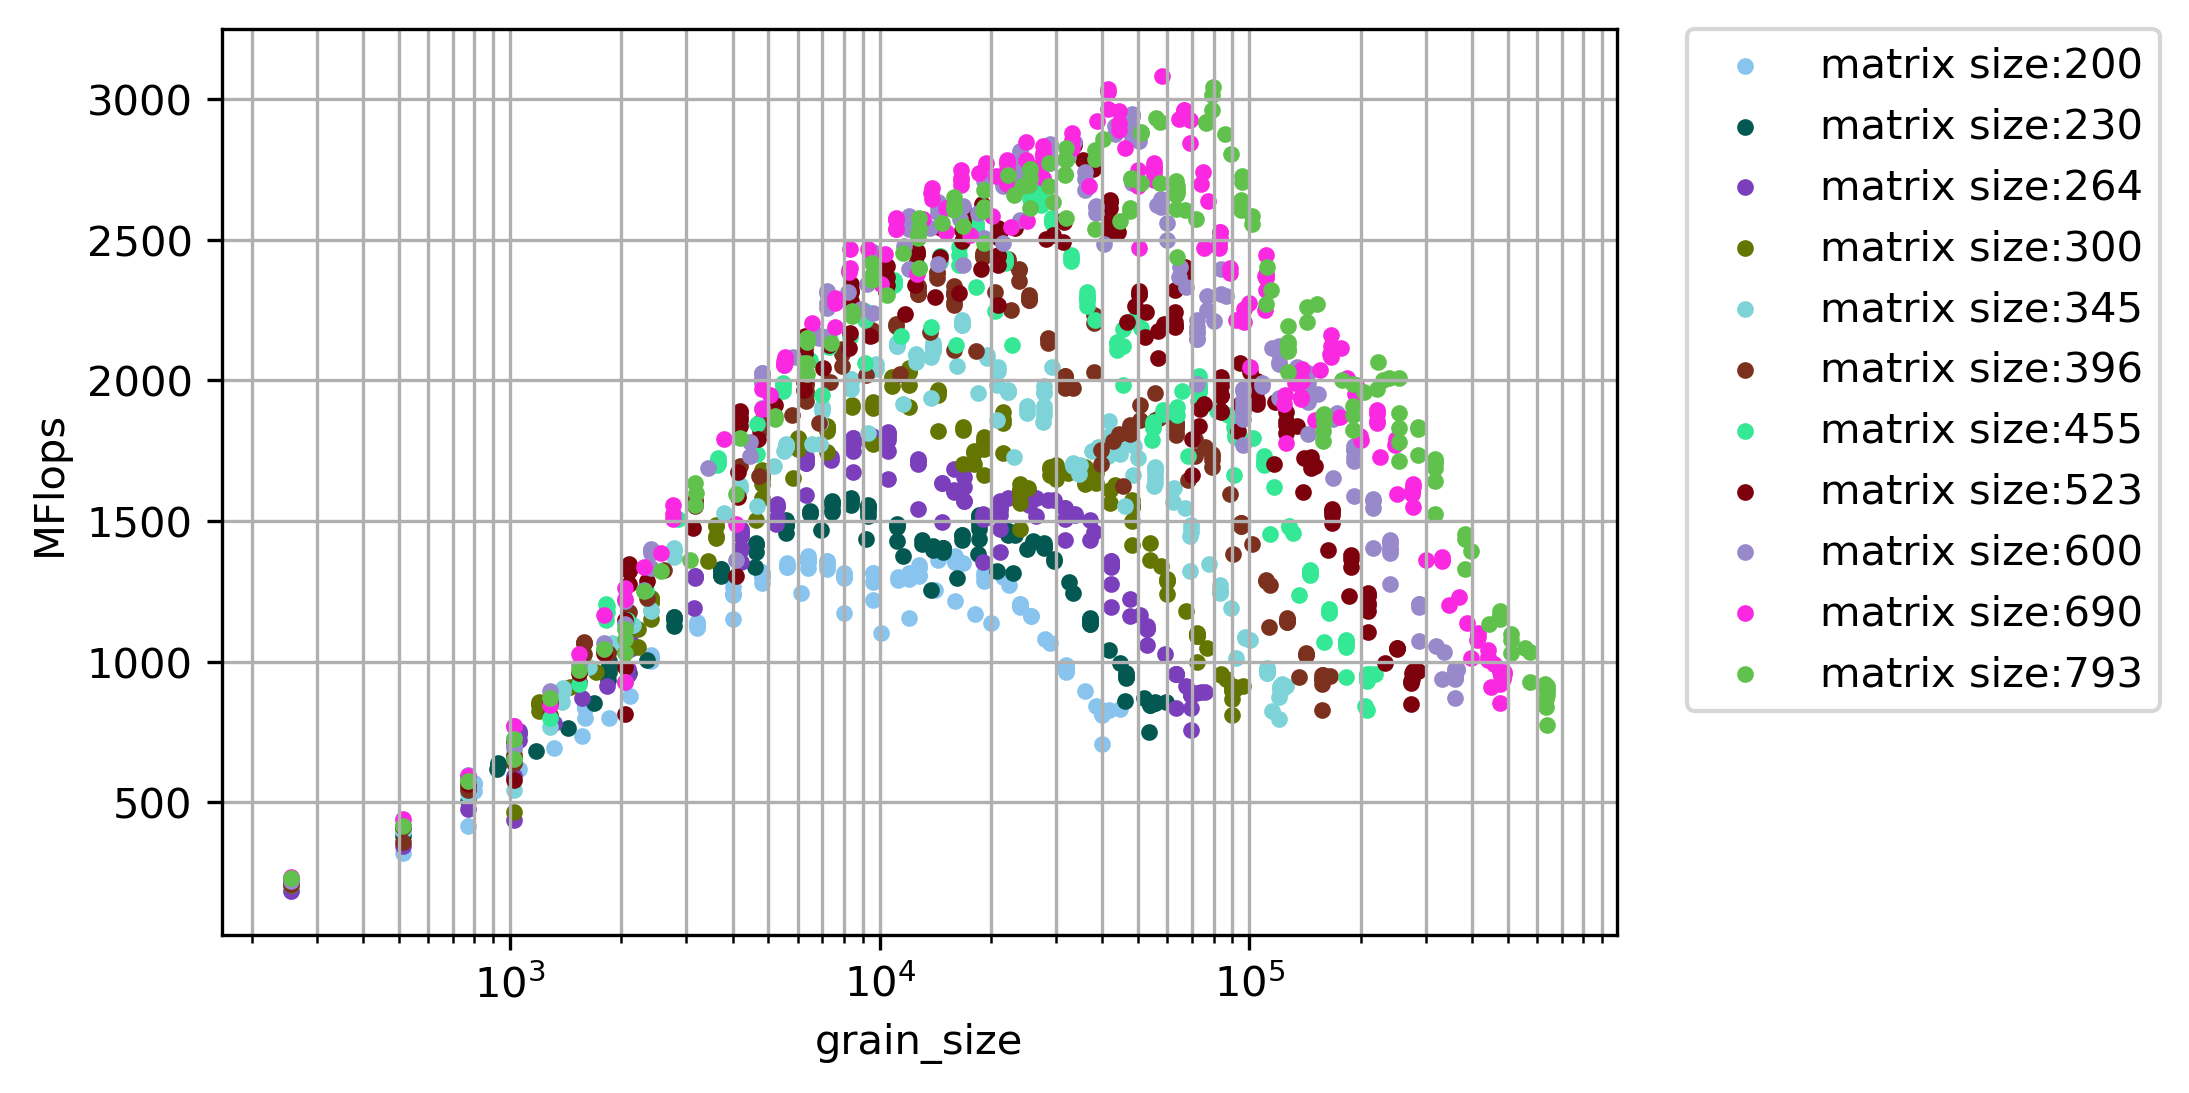
\includegraphics[scale=.75]{images/fig11.png}			
	\caption{Throughput vs. grain size graph obtained from running $DMATDMATADD$ benchmark  on $4$ cores.}
	\label{fig19}	
\end{figure} 


Moreover, Figure~\ref{fig20} shows how the predicted grain size range changes for different matrix sizes for each number of cores.
 
\vspace{\baselineskip}	
\begin{figure}[H]
	\centering
	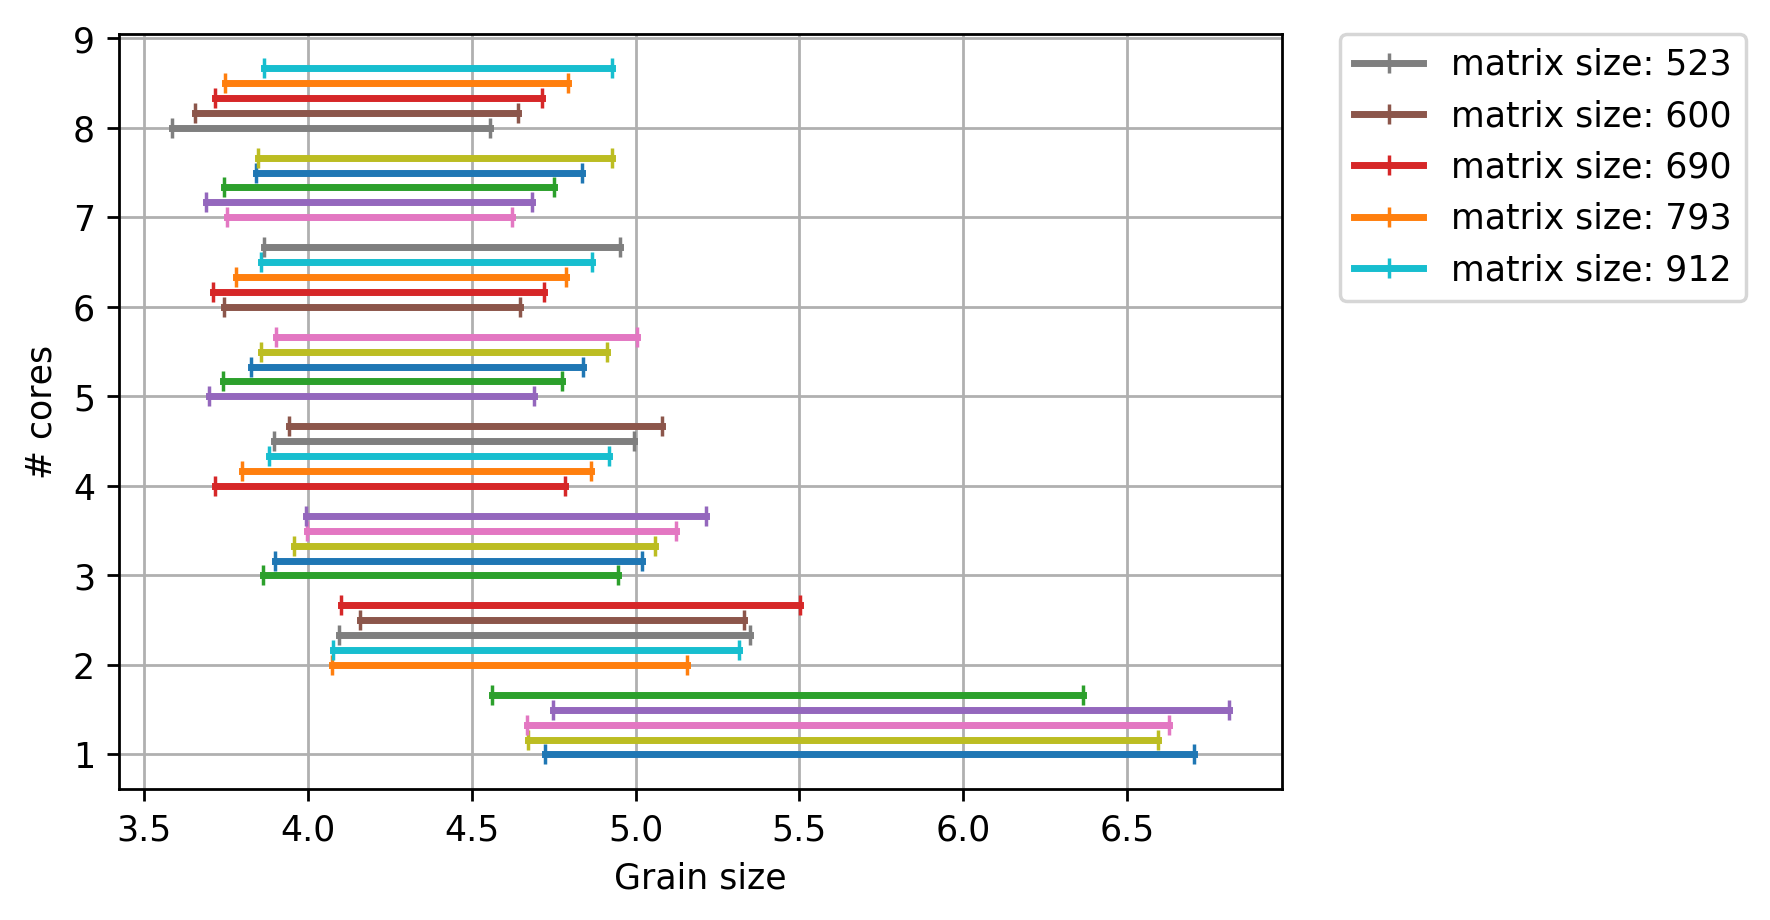
\includegraphics[scale=.5]{images/polyfit/fig_523-912_peak_range_all.png}

	\caption{The range of grain size within $10\%$ of the maximum performance of the fitted polynomial function for $DMATDMATADD$ benchmark for different number of cores for matrix size $523\times523$ to $912\times912$.}	
	\label{fig20}
\end{figure} 
\vspace{\baselineskip}	
Also, larger matrix sizes should be added to the experiments to validate the current results. 

\vspace{\baselineskip}	
\section{Generalization for complex expressions}
The whole study here was based on a simple matrix-matrix addition, and was validated on the same operation. We have been looking at the grain size as the key factor here, while the complexity of the operation has been included in the grain size. In the next step we need to add more benchmarks and study if the behavior is consistent for the other benchmarks. 
In addition to the operation, the number of matrices involved in the operation is also important, since it affects the threshold from which the matrices would not fit into the cache, which itself results in a performance degradation.


\vspace{\baselineskip}	
\section{Generalization for different architectures}
We are proposing here that once we have a generalized model, the parameters of the model are the factors that would change from one architecture to another. This, along with the cache specifications of the machines, should direct us toward fine tuning the performance for each architecture.
One option could be running a set of benchmarks at build time to find these parameters for each machine. Once these parameters are found, we would be able to use our models to find the best grain size for the specific expression we are evaluating, considering the matrix size and the number of cores.



